\documentclass[11pt,a4paper]{book}

% bibliography on the same page
% https://tex.stackexchange.com/questions/74296/to-have-no-pagebreak-before-bibliography
\usepackage{etoolbox}
\patchcmd{\thebibliography}{\chapter*}{\section*}{}{}

\usepackage{ceteiep_dsa_notes_whitebg}

\addto\captionsgreek{\renewcommand{\chaptername}{Εργαστήριο}}

\title{Δομές Δεδομένων και Αλγόριθμοι \\ ΜΕΡΟΣ Γ' \\ Εργαστήριο (C++)\\ Τ.Ε.Ι. Ηπείρου - Τμήμα Μηχανικών Πληροφορικής Τ.Ε.}
\author{Χρήστος Γκόγκος }
\date{Άρτα - 2017}

\begin{document}
% \frontmatter
\maketitle
% \tableofcontents
\mainmatter

\setcounter{chapter}{6} 
% Εργαστήριο 7
\chapter{Κατακερματισμός, δομές κατακερματισμού στην STL}
\section{Εισαγωγή}
Ο κατακερματισμός (hashing) αποτελεί μια από τις βασικές τεχνικές στη επιστήμη των υπολογιστών. Χρησιμοποιείται στις δομές δεδομένων αλλά και σε άλλα πεδία της πληροφορικής όπως η κρυπτογραφία. Στο εργαστήριο αυτό θα παρουσιαστεί η δομή δεδομένων πίνακας κατακερματισμού χρησιμοποιώντας δύο διαδεδομένες υλοποιήσεις: την ανοικτή διευθυνσιοδότηση και την υλοποίηση με αλυσίδες. Επιπλέον, θα παρουσιαστούν δομές της STL όπως η unordered\_set και η unordered\_map οι οποίες στηρίζονται στην τεχνική του κατακερματισμού. Ο κώδικας όλων των παραδειγμάτων, όπως και στα προηγούμενα εργαστήρια, βρίσκεται στο \href{https://github.com/chgogos/ceteiep_dsa}{https://github.com/chgogos/ceteiep\_dsa}.

\section{Τι είναι ο κατακερματισμός;}
Ο κατακερματισμός είναι μια μέθοδος που επιτυγχάνει ταχύτατη αποθήκευση, αναζήτηση και διαγραφή δεδομένων. Σε ένα σύστημα κατακερματισμού τα δεδομένα αποθηκεύονται σε έναν πίνακα που ονομάζεται πίνακας κατακερματισμού (hash table). Θεωρώντας ότι τα δεδομένα είναι εγγραφές που αποτελούνται από ζεύγη τιμών της μορφής κλειδί-τιμή, η βασική ιδέα είναι, ότι εφαρμόζοντας στο κλειδί κάθε εγγραφής που πρόκειται να αποθηκευτεί ή να αναζητηθεί τη λεγόμενη συνάρτηση κατακερματισμού (hash function), προσδιορίζεται μονοσήμαντα η θέση του πίνακα στην οποία τοποθετούνται τα δεδομένα της εγγραφής. Η συνάρτηση κατακερματισμού αναλαμβάνει να αντιστοιχήσει έναν μεγάλο αριθμό ή ένα λεκτικό σε ένα μικρό ακέραιο που χρησιμοποιείται ως δείκτης στον πίνακα κατακερματισμού.

\begin{figure}[ht]
\centering
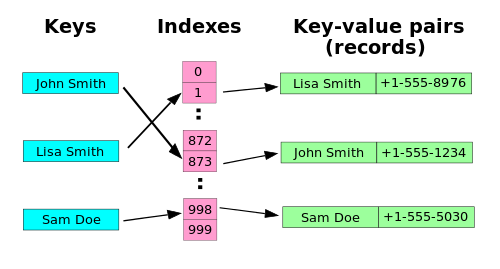
\includegraphics[width=100mm]{HASHTB08.png}
\caption{Κατακερματισμός εγγραφών σε πίνακα κατακερματισμού \cite{wiki_hashtables}}
\label{fig:hashtable1}
\end{figure}

Μια καλή συνάρτηση κατακερματισμού θα πρέπει να κατανέμει τα κλειδιά στα κελιά του πίνακα κατακερματισμού όσο πιο ομοιόμορφα γίνεται και να είναι εύκολο να υπολογιστεί. Επίσης, είναι επιθυμητό το παραγόμενο αποτέλεσμα από τη συνάρτηση κατακερματισμού να εξαρτάται από το κλειδί στο σύνολό του.

Στον κώδικα που ακολουθεί παρουσιάζονται τέσσερις συναρτήσεις κατακερματισμού κάθε μία από τις οποίες δέχεται ένα λεκτικό και επιστρέφει έναν ακέραιο αριθμό. Στις συναρτήσεις hash2 και hash3 γίνεται χρήση τελεστών που εφαρμόζονται σε δυαδικές τιμές (bitwise operators). Ειδικότερα χρησιμοποιούνται οι τελεστές $<<$ (αριστερή ολίσθηση), $>>$ (δεξιά ολίσθηση) και $\hat{}$ (xor - αποκλειστικό ή).

\lstinputlisting[caption = Διάφορες συναρτήσεις κατακερματισμού (hashes.cpp)]{lab07/hashes.cpp}

\lstinputlisting[caption = Παραδείγματα κλήσεων συναρτήσεων κατακερματισμού (hashes\_ex1.cpp)]{lab07/hashes_ex1.cpp}

\lstinputlisting[style=DOS]{lab07/hashes_ex1.out}


Οι πίνακες κατακερματισμού είναι ιδιαίτερα κατάλληλοι για εφαρμογές στις οποίες πραγματοποιούνται συχνές αναζητήσεις εγγραφών με δεδομένες τιμές κλειδιών. Οι βασικές λειτουργίες που υποστηρίζονται σε έναν πίνακα κατακερματισμού είναι η εισαγωγή (insert), η αναζήτηση (get) και η διαγραφή (erase). Και οι τρεις αυτές λειτουργίες παρέχονται σε χρόνο $O(1)$ κατά μέσο όρο προσφέροντας ταχύτερη υλοποίηση σε σχέση με άλλες υλοποιήσεις όπως για παράδειγμα τα ισοζυγισμένα δυαδικά δένδρα αναζήτησης που παρέχουν τις ίδιες λειτουργίες σε χρόνο $O(log n)$. 

Ωστόσο, οι πίνακες κατακερματισμού έχουν και μειονεκτήματα καθώς είναι δύσκολο να επεκταθούν από τη στιγμή που έχουν δημιουργηθεί και μετά. Επίσης, η απόδοση των πινάκων κατακερματισμού υποβαθμίζεται καθώς οι θέσεις τους γεμίζουν με στοιχεία. Συνεπώς, εφόσον ο προγραμματιστής προχωρήσει στη δική του υλοποίηση ενός πίνακα κατακερματισμού είτε θα πρέπει να γνωρίζει εκ των προτέρων το πλήθος των στοιχείων που πρόκειται να αποθηκευτούν είτε όταν αυτό απαιτηθεί να υπάρχει πρόβλεψη έτσι ώστε τα δεδομένα να μεταφέρονται σε μεγαλύτερο πίνακα κατακερματισμού.

Στις περισσότερες εφαρμογές υπάρχουν πολύ περισσότερα πιθανά κλειδιά εγγραφών από ότι θέσεις στο πίνακα κατακερματισμού. Αν για δύο ή περισσότερα κλειδιά η εφαρμογή της συνάρτησης κατακερματισμού επιστρέφει το ίδιο αποτέλεσμα τότε λέμε ότι συμβαίνει σύγκρουση (collision) η οποία θα πρέπει να διευθετηθεί με κάποιο τρόπο. Ο ακόλουθος κώδικας μετρά το πλήθος των συγκρούσεων που συμβαίνουν καθώς δημιουργούνται hashes για ένα σύνολο 2.000 κλειδιών αλφαριθμητικού τύπου.


\lstinputlisting[caption = Δημιουργία τυχαίων λεκτικών (random\_strings.cpp)]{lab07/random_strings.cpp}

\lstinputlisting[caption = Συγκρούσεις (hashes\_ex2.cpp)]{lab07/hashes_ex2.cpp}

\lstinputlisting[style=DOS]{lab07/hashes_ex2.out}

Γενικότερα, σε έναν πίνακα κατακερματισμού, η εύρεση μιας εγγραφής με κλειδί key είναι μια διαδικασία δύο βημάτων:
\begin{itemize}[noitemsep]
\item Εφαρμογή της συνάρτησης κατακερματισμού στο κλειδί της εγγραφής.
\item Ξεκινώντας από την θέση που υποδεικνύει η συνάρτηση κατακερματισμού στον πίνακα κατακερματισμού, εντοπισμός της εγγραφής που περιέχει το ζητούμενο κλειδί (ενδεχόμενα θα χρειαστεί να εφαρμοστεί κάποιος μηχανισμός διευθέτησης συγκρούσεων). 
\end{itemize}

Οι βασικοί μηχανισμοί επίλυσης των συγκρούσεων είναι η ανοικτή διευθυνσιοδότηση και ο κατακερματισμός με αλυσίδες.

\subsection{Ανοικτή διευθυνσιοδότηση}
Στην ανοικτή διευθυνσιοδότηση (open addressing, closed hashing) όλα τα δεδομένα αποθηκεύονται απευθείας στον πίνακα κατακερματισμού. Αν συμβεί σύγκρουση τότε ελέγχεται αν κάποιο από τα υπόλοιπα κελιά είναι διαθέσιμο και η εγγραφή τοποθετείται εκεί. Συνεπώς, θα πρέπει το μέγεθος του hashtable να είναι μεγαλύτερο ή ίσο από το πλήθος των στοιχείων που πρόκειται να αποθηκευτούν σε αυτό. Θα πρέπει να σημειωθεί ότι η απόδοση της ανοικτής διευθυνσιοδότησης μειώνεται κατακόρυφα σε περίπτωση που το hashtable είναι σχεδόν γεμάτο. 

Αν το πλήθος των κελιών είναι $m$ και το πλήθος των εγγραφών είναι $n$ τότε το πηλίκο $a=\frac{n}{m}$ που ονομάζεται παράγοντας φόρτωσης (load factor) καθορίζει σημαντικά την απόδοση του hashtable. Ο παράγοντας φόρτωσης στην περίπτωση της ανοικτής διευθυνσιοδότησης δεν μπορεί να είναι μεγαλύτερος της μονάδας.

Υπάρχουν πολλές παραλλαγές της ανοικτής διευθυνσιοδότησης που σχετίζονται με τον τρόπο που σε περίπτωση σύγκρουσης επιλέγεται το επόμενο κελί που εξετάζεται αν είναι ελεύθερο προκειμένου να τοποθετηθούν εκεί τα δεδομένα της εγγραφής. Αν εξετάζεται το αμέσως επόμενο στη σειρά κελί και μέχρι να βρεθεί το πρώτο διαθέσιμο, ξεκινώντας από την αρχή του πίνακα αν βρεθεί στο τέλος, τότε η μέθοδος ονομάζεται γραμμική ανίχνευση (linear probing). Άλλες διαδεδομένες μέθοδοι είναι η τετραγωνική ανίχνευση (quadratic probing) και ο διπλός κατακερματισμός (double hashing) \cite{visualalgo_hashtables}.

\begin{figure}[ht]
\centering
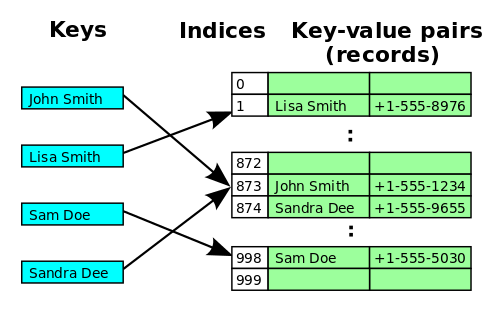
\includegraphics[width=100mm]{HASHTB12.png}
\caption{Κατακερματισμός εγγραφών με ανοικτή διευθυνσιοδότηση και γραμμική ανίχνευση \cite{wiki_hashtables}}
\label{fig:hashtable2}
\end{figure}

Στη συνέχεια ακολουθεί μια υλοποίηση ενός πίνακα κατακερματισμού με ανοικτή διευθυνσιοδότηση και γραμμική ανίχνευση. Στον πίνακα κατακερματισμού τοποθετούνται εγγραφές με κλειδιά και τιμές αλφαριθμητικού τύπου. 

\lstinputlisting[label={lst:open_addressing},caption={Ανοικτή διευθυνσιοδότηση (open\_addressing.cpp)}]{lab07/open_addressing.cpp}

\lstinputlisting[style=DOS]{lab07/open_addressing.out}

\subsection{Κατακερματισμός με αλυσίδες}
Στον κατακερματισμό με αλυσίδες (separate chaining) οι εγγραφές αποθηκεύονται σε συνδεδεμένες λίστες κάθε μια από τις οποίες είναι προσαρτημένες στα κελιά ενός hashtable. Συνεπώς, η απόδοση των αναζητήσεων εξαρτάται από τα μήκη των συνδεδεμένων λιστών. Αν η συνάρτηση κατακερματισμού κατανέμει τα $n$ κλειδιά ανάμεσα στα $m$ κελιά ομοιόμορφα τότε κάθε λίστα θα έχει μήκος $\frac{n}{m}$. O παράγοντας φόρτωσης, $a=\frac{n}{m}$, στον κατακερματισμό με αλυσίδες δεν θα πρέπει να απέχει πολύ από την μονάδα. Πολύ μικρό load factor σημαίνει ότι υπάρχουν πολλές κενές λίστες και συνεπώς δεν γίνεται αποδοτική χρήση του χώρου ενώ μεγάλο load factor σημαίνει μακριές συνδεδεμένες λίστες και μεγαλύτεροι χρόνοι αναζήτησης. 

\begin{figure}[ht]
\centering
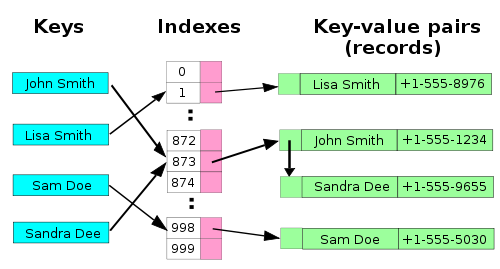
\includegraphics[width=100mm]{HASHTB32.png}
\caption{Κατακερματισμός εγγραφών με αλυσίδες \cite{wiki_hashtables}}
\label{fig:hashtable3}
\end{figure}

Στη συνέχεια ακολουθεί μια υλοποίηση ενός πίνακα κατακερματισμού με κατακερματισμό με αλυσίδες. Για τις συνδεδεμένες λίστες χρησιμοποιείται η λίστα std::list.

\lstinputlisting[caption = Κατακερματισμός με αλυσίδες (separate\_chaining.cpp)]{lab07/separate_chaining.cpp}

\lstinputlisting[style=DOS]{lab07/separate_chaining.out}

Περισσότερες πληροφορίες σχετικά με τον κατακερματισμό και την υλοποίηση πινάκων κατακερματισμού μπορούν να βρεθούν στις αναφορές \cite{pumpkin_hashtables}, \cite{hackerearth_hashtables}.

\section{Κατακερματισμός με την STL}
Η STL διαθέτει την κλάση std::hash που μπορεί να χρησιμοποιηθεί για την επιστροφή hash τιμών για διάφορους τύπους δεδομένων. Στον ακόλουθο κώδικα παρουσιάζεται η χρήση της std::hash.

\lstinputlisting[caption = Παράδειγμα χρήσης της std::hash (stl\_hash.cpp)]{lab07/stl_hash.cpp}

\lstinputlisting[style=DOS]{lab07/stl_hash.out}
 

Επιπλέον, η STL υποστηρίζει δύο βασικές δομές κατακερματισμού το std::unordered\_set και το std::unordered\_map. Το std::unordered\_set υλοποιείται ως ένας πίνακας κατακερματισμού και μπορεί να περιέχει τιμές (κλειδιά) οποιουδήποτε τύπου οι οποίες γίνονται hash σε διάφορες θέσεις του πίνακα κατακερματισμού. Κατά μέσο όρο, οι λειτουργίες σε ένα std::unordered\_set (εύρεση, εισαγωγή και διαγραφή κλειδιού) πραγματοποιούνται σε σταθερό χρόνο O(1). Ένα std::unordered\_set δεν περιέχει διπλότυπα, ενώ αν υπάρχει αυτή η ανάγκη τότε μπορεί να χρησιμοποιηθεί το std::unordered\_multiset. 

Στον κώδικα που ακολουθεί οι χαρακτήρες ενός λεκτικού εισάγονται ένας προς ένας σε ένα std::unordered\_set έτσι ώστε να υπολογιστεί το πλήθος των διακριτών χαρακτήρων ενός λεκτικού.

\lstinputlisting[caption = Παράδειγμα χρήσης του std::unordered\_set (stl\_unordered\_set.cpp)]{lab07/stl_unordered_set.cpp}

\lstinputlisting[style=DOS]{lab07/stl_unordered_set.out}

To std::unordered\_map αποθηκεύει ζεύγη (κλειδί-τιμή). Το κλειδί αναγνωριζει με μοναδικό τρόπο το κάθε ζεύγος και γίνεται hash σε συγκεκριμένη θέση του πίνακα κατακερματισμού. Όπως και στο std::unordered\_set. κατά μέσο όρο, οι λειτουργίες σε ένα std::unordered\_map πραγματοποιούνται σε σταθερό χρόνο O(1). Η ανάθεση τιμής σε κλειδί μπορεί να γίνει με τους τελεστές = και [], ενώ το πέρασμα από τις τιμές ενός std::unordered\_map μπορεί να γίνει με  iterator ή με range for.
 
\lstinputlisting[caption = Παράδειγμα χρήσης του std::unordered\_map (stl\_unordered\_map.cpp)]{lab07/stl_unordered_map.cpp}

\lstinputlisting[style=DOS]{lab07/stl_unordered_map.out}

%\section{Κατακερματισμός και κρυπτογράφηση}
%
%\section{Bloom filters}
%A Bloom filter is a space-efficient probabilistic data structure, conceived by Burton Howard Bloom in 1970, that is used to test whether an element is a member of a set. False positive matches are possible, but false negatives are not – in other words, a query returns either "possibly in set" or "definitely not in set". Elements can be added to the set, but not removed (though this can be addressed with a "counting" filter); the more elements that are added to the set, the larger the probability of false positives.

\section{Παραδείγματα}

\subsection{Παράδειγμα 1}
Έστω μια επιχείρηση η οποία επιθυμεί να αποθηκεύσει τα στοιχεία των υπαλλήλων της (όνομα, διεύθυνση) σε μια δομή έτσι ώστε με βάση το όνομα του υπαλλήλου να επιτυγχάνει τη γρήγορη ανάκληση των υπόλοιπων στοιχείων των υπαλλήλων. Στη συνέχεια παρουσιάζεται η υλοποίηση ενός πίνακα κατακερματισμού στον οποίο κλειδί θεωρείται το όνομα του υπαλλήλου και η επίλυση των συγκρούσεων πραγματοποιείται με ανοικτή διευθυνσιοδότηση (open addressing) και γραμμική ανίχνευση (linear probing). Καθώς δεν υπάρχει η ανάγκη διαγραφής τιμών από τον πίνακα κατακερματισμού παρουσιάζεται μια απλούστερη υλοποίηση σε σχέση με αυτή που παρουσιάστηκε στον κώδικα \ref{lst:open_addressing}. Ο πίνακας κατακερματισμού μπορεί να δεχθεί το πολύ 100.000 εγγραφές υπαλλήλων. Στο παράδειγμα χρονομετρείται η εκτέλεση για 20.000, 30.000 και 80.000 υπαλλήλους. Παρατηρείται ότι λόγω των συγκρούσεων καθώς ο συντελεστής φόρτωσης του πίνακα κατακερματισμού αυξάνεται η απόδοση της δομής υποβαθμίζεται.

\lstinputlisting[caption = Yλοποίηση πίνακα κατακερματισμού για γρήγορη αποθήκευση και αναζήτηση εγγραφών (lab07\_ex1.cpp)]{lab07/lab07_ex1.cpp}

\lstinputlisting[style=DOS]{lab07/lab07_ex1.out}

\subsection{Παράδειγμα 2}
Στο παράδειγμα αυτό παρουσιάζεται η λύση του ίδιου προβλήματος με το παράδειγμα 1 με τη διαφορά ότι πλέον χρησιμοποιείται η δομή std::unordered\_map της STL.

\lstinputlisting[caption = Γρήγορη αποθήκευση και αναζήτηση εγγραφών με τη χρήση της std::unordered\_map (lab07\_ex2.cpp)]{lab07/lab07_ex2.cpp}

\lstinputlisting[style=DOS]{lab07/lab07_ex2.out}

\subsection{Παράδειγμα 3}
Στο παράδειγμα αυτό εξετάζονται τέσσερις διαφορετικοί τρόποι με τους οποίους ελέγχεται για ένα μεγάλο πλήθος τιμών (5.000.000) πόσες από αυτές περιέχονται σε ένα δεδομένο σύνολο 1.000 τιμών. Οι τιμές είναι ακέραιες και επιλέγονται με τυχαίο τρόπο στο διάστημα [0,100.000]. Ο χρόνος που απαιτεί η κάθε προσέγγιση χρονομετρείται.
\begin{itemize}[noitemsep]
\item Η πρώτη προσέγγιση (scenario1) χρησιμοποιεί ένα vector για να αποθηκεύσει το σύνολο των 1.000 τυχαίων ακεραίων τιμών και αναζητά σειριακά κάθε τιμή στο vector. 
\item Η δεύτερη προσέγγιση (scenario2) χρησιμοποιεί επίσης ένα vector για να αποθηκεύσει το σύνολο των 1.000 τυχαίων ακεραίων τιμών, τις ταξινομεί και αναζητά κάθε τιμή στο ταξινομημένο vector. 
\item Η τρίτη προσέγγιση (scenario3) αποθηκεύει τις 1.000 τυχαίες ακεραίες τιμές σε ένα std::set (υλοποιείται στην STL ως δυαδικό δένδρο αναζήτησης) και αναζητά κάθε τιμή σε αυτό. 
\item Η τέταρτη προσέγγιση (scenario4) αποθηκεύει τις 1.000 τυχαίες ακεραίες τιμές σε ένα std::unordered\_set (υλοποιείται στην STL ως πίνακας κατακερματισμού) και αναζητά κάθε τιμή σε αυτό.
%\item Η πέμπτη προσέγγιση (scenario5) υλοποιεί ένα Bloom filter που χρησιμοποιεί ως βασική δομή ένα σύνολο δυαδικών ψηφίων με μέγεθος 10.001. 
\end{itemize}

\lstinputlisting[caption = Έλεγχος ύπαρξης τιμών σε ένα σύνολο τιμών (lab07\_ex3.cpp)]{lab07/lab07_ex3.cpp}

\lstinputlisting[style=DOS]{lab07/lab07_ex3.out}

\section{Ασκήσεις}
\begin{enumerate}
\item Γράψτε μια συνάρτηση που να δέχεται έναν πίνακα ακεραίων Α και έναν ακέραιο αριθμό sum και να βρίσκει το πλήθος από όλα τα ζεύγη τιμών του Α που το άθροισμά τους είναι ίσο με sum.
\item Γράψτε ένα πρόγραμμα που για ένα λεκτικό που θα δέχεται ως είσοδο, να επιστρέφει το χαρακτήρα (γράμματα κεφαλαία, γράμματα πεζά, ψηφία, σύμβολα) που εμφανίζεται περισσότερες φορές καθώς και πόσες φορές εμφανίζεται στο λεκτικό.
\item Γράψτε μια συνάρτηση που να δέχεται έναν πίνακα ακεραίων Α και έναν ακέραιο αριθμό Κ και να βρίσκει τη μεγαλύτερη σε μήκος υποακολουθία στοιχείων του Α που έχει άθροισμα ίσο με Κ.
\item Γράψτε ένα πρόγραμμα που να δέχεται μια λέξη και να βρίσκει γρήγορα όλες τις άλλες έγκυρες λέξεις που είναι αναγραμματισμοί της λέξης που δόθηκε. Θεωρείστε ότι έχετε δεδομένο ένα αρχείο κειμένου με όλες τις έγκυρες λέξεις (words.txt), μια ανά γραμμή.
\end{enumerate}

\begin{thebibliography}{9}
\bibitem{wiki_hashtables}
Wikibooks, Data Structures - Hash Tables \href{https://en.wikibooks.org/wiki/Data_Structures/Hash_Tables}{https://en.wikibooks.org/wiki/Data\_Structures/Hash\_Tables}

\bibitem{pumpkin_hashtables}
C++ tutorial: Intro to Hash Tables,
\href{https://pumpkinprogrammerdotcom4.wordpress.com/2014/06/21/c-tutorial-intro-to-hash-tables/}{https://pumpkinprogrammerdotcom4.wordpress.com/2014/06/21/c-tutorial-intro-to-hash-tables/}

\bibitem{hackerearth_hashtables}
HackerEarth, Basics of Hash Tables, \href{https://www.hackerearth.com/practice/data-structures/hash-tables/basics-of-hash-tables/tutorial/}{https://www.hackerearth.com/practice/data-structures/hash-tables/basics-of-hash-tables/tutorial/}

\bibitem{visualalgo_hashtables}
VisualAlgo.net Open Addressing (LP, QP, DH) and Separate Chaining Visualization, \href{https://visualgo.net/en/hashtable}{https://visualgo.net/en/hashtable}

\end{thebibliography}



% Εργαστήριο 8
\chapter{Γραφήματα}
\section{Εισαγωγή}
Τα γραφήματα είναι δομές δεδομένων που συναντώνται συχνά κατά την επίλυση προβλημάτων. Η ευχέρεια προγραμματισμού αλγορίθμων που εφαρμόζονται πάνω σε γραφήματα είναι ουσιώδης. Καθώς μάλιστα συχνά ανακύπτουν προβλήματα για τα οποία έχουν διατυπωθεί αλγόριθμοι αποδοτικής επίλυσής τους η γνώση των αλγορίθμων αυτών αποδεικνύεται ισχυρός σύμμαχος στην επίλυση δύσκολων προβλημάτων. 

\section{Γραφήματα}
Ένα γράφημα ή γράφος (graph) είναι ένα σύνολο από σημεία που ονομάζονται κορυφές (vertices) ή κόμβοι (nodes) για τα οποία ισχύει ότι κάποια από αυτά είναι συνδεδεμένα απευθείας μεταξύ τους με τμήματα γραμμών που ονομάζονται ακμές (edges ή arcs). Συνήθως ένα γράφημα συμβολίζεται ως $G=(V,E)$ όπου $V$ είναι το σύνολο των κορυφών και $E$ είναι το σύνολο των ακμών.

Αν οι ακμές δεν έχουν κατεύθυνση τότε το γράφημα ονομάζεται μη κατευθυνόμενο (undirected) ενώ σε άλλη περίπτωση ονομάζεται κατευθυνόμενο (directed). Ένα πλήρες γράφημα (που όλες οι κορυφές συνδέονται απευθείας με όλες τις άλλες κορυφές) έχει $\frac{|V||V-1|}{2}$ ακμές ($|V|$ είναι το πλήθος των κορυφών του γραφήματος). Αν σε κάθε ακμή αντιστοιχεί μια τιμή τότε το γράφημα λέγεται γράφημα με βάρη. Το γράφημα του σχήματος \ref{fig:undirected_graph1} είναι ένα μη κατευθυνόμενο γράφημα με βάρη. 

\begin{figure}[ht]
	\centering
	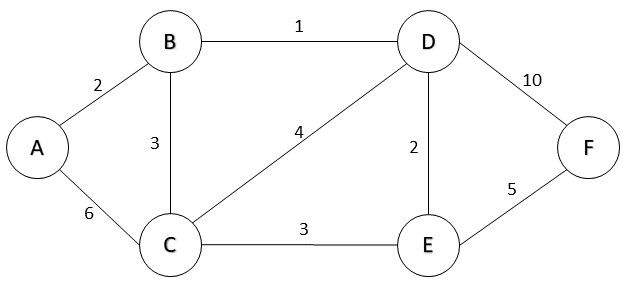
\includegraphics[width=100mm]{undirected_graph1.png}
	\caption{Ένα μη κατευθυνόμενο γράφημα 6 κορυφών και 9 ακμών με βάρη στις ακμές του}
	\label{fig:undirected_graph1}
\end{figure}

Ένα γράφημα λέγεται συνεκτικό αν για δύο οποιεσδήποτε κορυφές του υπάρχει μονοπάτι που τις συνδέει. Αν ένα γράφημα δεν είναι συνεκτικό τότε αποτελείται από επιμέρους συνεκτικά γραφήματα τα οποία λέγονται συνιστώσες. Είναι προφανές ότι ένα συνεκτικό γράφημα έχει μόνο μια συνιστώσα.

\subsection{Αναπαράσταση γραφημάτων}
Δύο διαδεδομένοι τρόποι αναπαράστασης γραφημάτων είναι οι πίνακες γειτνίασης (adjacency matrices) και οι λίστες γειτνίασης (adjacency lists).

Στους πίνακες γειτνίασης διατηρείται ένας δισδιάστατος πίνακας $n \times n$ όπου $n$ είναι το πλήθος των κορυφών του γραφήματος. Για κάθε ακμή του γραφήματος που συνενώνει την κορυφή $i$ με την κορυφή $j$ εισάγεται στη θέση $i,j$ του πίνακα το βάρος της ακμής αν το γράφημα είναι με βάρη ενώ αν δεν υπάρχουν βάρη τότε εισάγεται η τιμή 1. Όλα τα υπόλοιπα στοιχεία του πίνακα λαμβάνουν την τιμή 0. Για παράδειγμα η πληροφορία του γραφήματος για το σχήμα \ref{fig:undirected_graph1} διατηρείται όπως φαίνεται στον πίνακα \ref{tbl:adjacency_table}.

% Please add the following required packages to your document preamble:
% \usepackage[table,xcdraw]{xcolor}
% If you use beamer only pass "xcolor=table" option, i.e. \documentclass[xcolor=table]{beamer}
\begin{table}[ht]
	\centering
	\begin{tabular}{|
		>{\columncolor[HTML]{C0C0C0}}l |c|c|c|c|c|c|}
		\hline
		\cellcolor[HTML]{FFFFFF} & \cellcolor[HTML]{C0C0C0} A & \cellcolor[HTML]{C0C0C0} B & \cellcolor[HTML]{C0C0C0} C & \cellcolor[HTML]{C0C0C0}D & \cellcolor[HTML]{C0C0C0} E & \cellcolor[HTML]{C0C0C0} F \\ \hline
		A                        & 0                          & 2                          & 6                          & 0                         & 0                          & 0                          \\ \hline
		B                        & 2                          & 0                          & 3                          & 1                         & 0                          & 0                          \\ \hline
		C                        & 6                          & 3                          & 0                          & 4                         & 3                          & 0                          \\ \hline
		D                        & 0                          & 1                          & 4                          & 0                         & 2                          & 10                         \\ \hline
		E                        & 0                          & 0                          & 3                          & 2                         & 0                          & 5                          \\ \hline
		F                        & 0                          & 0                          & 0                          & 10                        & 5                          & 0                          \\ \hline
	\end{tabular}
	\caption{Πίνακας γειτνίασης για το σχήμα \ref{fig:undirected_graph1}}
    \label{tbl:adjacency_table}
\end{table}

Στις λίστες γειτνίασης διατηρούνται λίστες που περιέχουν για κάθε κορυφή όλη την πληροφορία των συνδέσεών της με τους γειτονικούς της κόμβους. Για παράδειγμα το γράφημα του σχήματος \ref{fig:undirected_graph1} μπορεί να αναπαρασταθεί με τις ακόλουθες 6 λίστες (μια ανά κορυφή). Κάθε στοιχείο της λίστας για την κορυφή $v$ είναι ένα ζεύγος τιμών $(w,u)$ και αναπαριστά μια ακμή από την κορυφή $v$ στην κορυφή $u$ με βάρος $w$, όπως φαίνεται στο πίνακα \ref{tbl:adjacency_list}.

\begin{table}[ht]
	\centering
	\begin{tabular}{|
		>{\columncolor[HTML]{C0C0C0}}l |c|}
		\hline
		A & (2,B), (6,C)                \\ \hline
		B & (2,A), (3,C), (1,D)         \\ \hline
		C & (6,A), (3,B), (4,D), (3,E)  \\ \hline
		D & (1,B), (4,C), (2,E), (10,F) \\ \hline
		E & (3,C), (2,D), (5,F)         \\ \hline
		F & (10,D), (5,E)               \\ \hline
	\end{tabular}
	\caption{Λίστα γειτνίασης για το σχήμα \ref{fig:undirected_graph1}}
	\label{tbl:adjacency_list}
\end{table}

Περισσότερα για τις αναπαραστάσεις γραφημάτων μπορούν να βρεθούν στις αναφορές \cite{g4g_graph_representations} και \cite{he_graph_representations}.

\subsection{Ανάγνωση δεδομένων γραφήματος από αρχείο}
Υπάρχουν πολλοί τρόποι με τους οποίους μπορούν να βρίσκονται καταγεγραμμένα τα δεδομένα ενός γραφήματος σε ένα αρχείο. Το αρχείο αυτό θα πρέπει να διαβαστεί έτσι ώστε να αναπαρασταθεί το γράφημα στη μνήμη του υπολογιστή. Στη συνέχεια παρουσιάζεται μια απλή μορφή αποτύπωσης κατευθυνόμενων με βάρη γραφημάτων χρησιμοποιώντας αρχεία απλού κειμένου. Σύμφωνα με αυτή τη μορφή για κάθε κορυφή του γραφήματος καταγράφεται σε ξεχωριστή γραμμή του αρχείου κειμένου το όνομά της ακολουθούμενο από ζεύγη τιμών, χωρισμένων με κόμματα, που αντιστοιχούν στις ακμές που ξεκινούν από τη συγκεκριμένη κορυφή. Στο κείμενο που ακολουθεί (graph1.txt) και το οποίο αφορά το γράφημα του σχήματος \ref{fig:undirected_graph1} η πρώτη γραμμή σημαίνει ότι η κορυφή Α συνδέεται με μια ακμή με βάρος 2 με την κορυφή B καθώς και με μια ακμή με βάρος 6 με την κορυφή C. Ανάλογα καταγράφεται η πληροφορία ακμών και για τις άλλες κορυφές.

\lstinputlisting[style=DOS]{lab08/graph1.txt}

Η ανάγνωση του αρχείου και η αναπαράσταση του γραφήματος ως λίστα γειτνίασης γίνεται με τη συνάρτηση read\_data που δίνεται στη συνέχεια όπου fn είναι το όνομα του αρχείου. Η συνάρτηση αυτή δημιουργεί ένα λεξικό (map) που αποτελείται από εγγραφές τύπου key-value. Σε κάθε εγγραφή το key είναι ένα λεκτικό με το όνομα μιας κορυφής ενώ το value είναι ένα διάνυσμα (vector) που περιέχει ζεύγη (pair<int,string>) στα οποία το πρώτο στοιχείο είναι ένας ακέραιος αριθμός που αναπαριστά το βάρος μιας ακμής ενώ το δεύτερο ένα λεκτικό με το όνομα της κορυφής στην οποία καταλήγει η ακμή από την κορυφή key. Ο κώδικας έχει ``σπάσει'' σε 3 αρχεία (graph.hpp, graph.cpp και graph\_ex1.cpp) έτσι ώστε να είναι ευκολότερη η επαναχρησιμοποίηση του. Η συνάρτηση print\_data εμφανίζει τα δεδομένα του γραφήματος.

\lstinputlisting[caption = header file με τις συναρτήσεις για ανάγνωση και εμφάνιση γραφημάτων (graph.hpp)]{lab08/graph.hpp}

\lstinputlisting[caption = source file με τις συναρτήσεις για ανάγνωση και εμφάνιση γραφημάτων (graph.cpp),multicols=2]{lab08/graph.cpp}

\lstinputlisting[caption = Ανάγνωση και εκτύπωση των δεδομένων του γραφήματος του σχήματος \ref{fig:undirected_graph1} (graph\_ex1.cpp)]{lab08/graph_ex1.cpp}

Η μεταγλώττιση και η εκτέλεση του κώδικα γίνεται με τις ακόλουθες εντολές:

\lstinputlisting[style=DOS]{lab08/compile_execute1.txt}

Η δε έξοδος που παράγεται είναι η ακόλουθη:

\lstinputlisting[style=DOS]{lab08/graph_ex1.out}

\subsection{Κατευθυνόμενα ακυκλικά γραφήματα}
Τα κατευθυνόμενα ακυκλικά γραφήματα (Directed Acyclic Graphs=DAGs) είναι γραφήματα για τα οποία δεν μπορεί να εντοπιστεί διαδρομή από μια κορυφή προς την ίδια. Στο σχήμα \ref{fig:dag1} παρουσιάζεται ένα γράφημα το οποίο δεν παρουσιάζει κύκλους. Αν για παράδειγμα υπήρχε μια ακόμα ακμή από την κορυφή E προς την κορυφή A τότε πλέον το γράφημα δεν θα ήταν DAG καθώς θα υπήρχε ο κύκλος A-C-E-A.

\begin{figure}[ht]
	\centering
	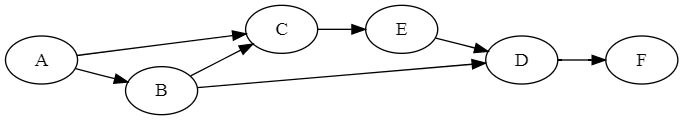
\includegraphics[width=120mm]{dag1.png}
	\caption{Ένα κατευθυνόμενο ακυκλικό γράφημα (DAG)}
	\label{fig:dag1}
\end{figure}

Τα DAGs χρησιμοποιούνται στη μοντελοποίηση πολλών καταστάσεων. Μπορούν για παράδειγμα να αναπαραστήσουν εργασίες που πρέπει να εκτελεστούν και για τις οποίες υπάρχουν εξαρτήσεις όπως για παράδειγμα ότι για να ξεκινήσει η εκτέλεση της εργασίας D θα πρέπει πρώτα να έχουν ολοκληρωθεί οι εργασίες B και E. 

\subsection{Σημαντικοί αλγόριθμοι γραφημάτων}
Υπάρχουν πολλοί αλγόριθμοι που εφαρμόζονται σε γραφήματα προκειμένου να επιλύσουν ενδιαφέροντα προβλήματα που ανακύπτουν σε πρακτικές εφαρμογές. Οι ακόλουθοι αλγόριθμοι είναι μερικοί από αυτούς:
\begin{itemize}[noitemsep]
	\item Αναζήτηση συντομότερων διαδρομών από μια κορυφή προς όλες τις άλλες κορυφές (Dijkstra). Ο αλγόριθμος αυτός θα αναλυθεί στη συνέχεια.
	\item Εύρεση μήκους συντομότερων διαδρομών για όλα τα ζεύγη κορυφών (Floyd Warshall) \cite{pa_floyd_warshall}.
	\item Αναζήτηση κατά βάθος (Depth First Search). Είναι αλγόριθμος διάσχισης γραφήματος ο οποίος ξεκινά από έναν κόμβο αφετηρία και επισκέπτεται όλους τους άλλους κόμβους που είναι προσβάσιμοι χρησιμοποιώντας της ακμές του γραφήματος. Λειτουργεί επεκτείνοντας μια διαδρομή όσο βρίσκει νέους κόμβους τους οποίους μπορεί να επισκεφθεί. Αν δεν βρίσκει νέους κόμβους οπισθοδρομεί και διερευνά άλλα τμήματα του γραφήματος.
	\item Αναζήτηση κατά πλάτος (Breadth First Search). Αλγόριθμος διάσχισης γραφήματος που ξεκινώντας από έναν κόμβο αφετηρία επισκέπτεται τους υπόλοιπους κόμβους σε αύξουσα σειρά βημάτων από την αφετηρία. Βήματα θεωρούνται οι μεταβάσεις από κορυφή σε κορυφή.
	\item Εντοπισμός ελάχιστου συνεκτικού (ή γεννητικού) δένδρου (Prim \cite{programiz_prim}, Kruskal \cite{programiz_kruskal}). Δεδομένου ενός γραφήματος, το πρόβλημα αφορά την εύρεση ενός δένδρου στο οποίο θα περιέχονται όλες οι κορυφές του γραφήματος ενώ οι ακμές του δένδρου θα είναι ένα υποσύνολο των ακμών του γραφήματος τέτοιο ώστε το άθροισμα των βαρών τους να είναι το ελάχιστο δυνατό.
	\item Τοπολογική ταξινόμηση (Topological Sort) \cite{g4g_topological_sort}. Ο αλγόριθμος τοπολογικής ταξινόμησης εφαρμόζεται σε DAGs και παράγει μια σειρά κορυφών του γραφήματος για την οποία ισχύει ότι για κάθε κατευθυνόμενη ακμή από την κορυφή $u$ στην κορυφή $v$ στη σειρά των κορυφών η κορυφή $u$ προηγείται της κορυφής $v$. Για παράδειγμα, για το DAG του σχήματος \ref{fig:dag1} αποτέλεσμα του αλγορίθμου είναι το A,B,C,E,D,F. Σε συνθετότερα γραφήματα μπορεί να υπάρχουν περισσότερες από μια τοπολογικές σειρές κορυφών για το γράφημα.
	\item Εντοπισμός κυκλωμάτων Euler (Eulerian circuit) \cite{dicretetext_euler_path}. Σε ένα γράφημα, διαδρομή Euler (Eulerian path) είναι μια διαδρομή που περνά από όλες τις ακμές του γραφήματος. Αν η διαδρομή αυτή ξεκινά και τερματίζει στην ίδια κορυφή τότε λέγεται κύκλωμα Euler. 
	\item Εντοπισμός ισχυρά συνδεδεμένων συνιστωσών (Strongly Connected Components) \cite{he_scc}. Ισχυρά συνδεδεμένες συνιστώσες υφίστανται μόνο σε κατευθυνόμενα γραφήματα. Ένα κατευθυνόμενο γράφημα είναι ισχυρά συνδεδεμένο όταν υπάρχει διαδρομή από κάθε κορυφή προς κάθε άλλη κορυφή. Ένα κατευθυνόμενο γράφημα μπορεί να σπάσει σε ισχυρά συνδεδεμένα υπογραφήματα. Τα υπογραφήματα αυτά αποτελούν τις ισχυρά συνδεδεμένες συνιστώσες του γραφήματος.
\end{itemize} 

 
\section{Αλγόριθμος του Dijkstra για εύρεση συντομότερων διαδρομών}
Ο αλγόριθμος δέχεται ως είσοδο ένα γράφημα $G=(V,E)$ και μια κορυφή του γραφήματος $s$ η οποία αποτελεί την αφετηρία. Υπολογίζει για όλες τις κορυφές $v \in V$ το μήκος του συντομότερου μονοπατιού από την κορυφή $s$ στην κορυφή $v$. Για να λειτουργήσει σωστά θα πρέπει κάθε ακμή να έχει μη αρνητικό βάρος. Αν το γράφημα περιέχει ακμές με αρνητικό βάρος τότε μπορεί να χρησιμοποιηθεί ο αλγόριθμος των Bellman-Ford \cite{brilliant_bellman_ford}.

\subsection{Περιγραφή του αλγορίθμου}
Ο αλγόριθμος εντοπίζει τις συντομότερες διαδρομές προς τις κορυφές του γραφήματος σε σειρά απόστασης από την κορυφή αφετηρία. Σε κάθε βήμα του αλγορίθμου η αφετηρία και οι ακμές προς τις κορυφές για τις οποίες έχει ήδη βρεθεί συντομότερο μονοπάτι σχηματίζουν το υποδένδρο $S$ του γραφήματος. Οι κορυφές που είναι προσπελάσιμες με 1 ακμή από το υποδένδρο $S$ είναι υποψήφιες να αποτελέσουν την επόμενη κορυφή που θα εισέλθει στο υποδένδρο. Επιλέγεται μεταξύ τους η κορυφή που βρίσκεται στη μικρότερη απόσταση από την αφετηρία. Για κάθε υποψήφια κορυφή $u$ υπολογίζεται το άθροισμα της απόστασής της από την πλησιέστερη κορυφή $v$ του δένδρου συν το μήκος της συντομότερης διαδρομής από την αφετηρία $s$ προς την κορυφή $v$. Στη συνέχεια επιλέγεται η κορυφή με το μικρότερο άθροισμα και προσαρτάται στο σύνολο των κορυφών που απαρτίζουν το υποδένδρο $S$. Για κάθε μία από τις υποψήφιες κορυφές που συνδέονται με μια ακμή με την κορυφή που επιλέχθηκε ενημερώνεται η απόστασή της από το υποδένδρο εφόσον προκύψει μικρότερη τιμή.

\paragraph{Ψευδοκώδικας}
Το σύνολο $S$ περιέχει τις κορυφές για τις οποίες έχει προσδιοριστεί η συντομότερη διαδρομή από την κορυφή $s$ ενώ το διάνυσμα $d$ περιέχει τις αποστάσεις από την κορυφή $s$ \\
1. Αρχικά $S={s}$, $d_s=0$ και για όλες τις κορυφές $i \neq s, d_i=\infty$ \\
2. Μέχρι να γίνει $S=V$ \\
3. Εντοπισμός του στοιχείου $v \notin S$ με τη μικρότερη τιμή $d_v$ και προσθήκη του στο $S$ \\
4. Για κάθε ακμή από την κορυφή $v$ στην κορυφή $u$ με βάρος $w$ ενημερώνεται η τιμή $d_u$ έτσι ώστε: \\
\centerline{$d_u=min(d_u, d_v+w)$}
5. Επιστροφή στο βήμα 2.

\paragraph{Εκτέλεση του αλγορίθμου}
Στη συνέχεια ακολουθεί παράδειγμα εκτέλεσης του αλγορίθμου για το γράφημα του σχήματος \ref{fig:undirected_graph1}.

\begin{table}[ht]
	\centering
	\label{tbl:dijkstra1}
	\begin{tabular}{|c|p{5cm}|}
		\hline
		$S=\{A\},d_A=0,d_B=2,d_C=6,d_D=\infty,d_E=\infty,d_F=\infty $   & Από το $S$ μπορούμε να φτάσουμε στις κορυφές B και C με μήκος διαδρομής 2 και 6 αντίστοιχα. Επιλέγεται η κορυφή B.                                                                                         \\ \hline
		$S=\{A,B\}, d_A=0, d_B=2, d_C=5, d_D=3, d_E=\infty, d_F=\infty$ & Από το $S$ μπορούμε να φτάσουμε στις κορυφές C και D με μήκος διαδρομής 5 και 3 αντίστοιχα. Επιλέγεται η κορυφή D.                                                                                         \\ \hline
		$S= \{A,B,D\},d_A=0,d_B=2,d_C=5,d_D=3,d_E=5,d_F=13$             & Από το $S$ μπορούμε να φτάσουμε στις κορυφές C, E και F με μήκος διαδρομής 5, 5 και 13 αντίστοιχα. Επιλέγεται (με τυχαίο τρόπο) ανάμεσα στις κορυφές C και E η κορυφή C. \\ \hline
		$S=\{A,B,D,C\},d_A=0,d_B=2,d_C=5,d_D=3,d_E=5,d_F=13$            & Από το $S$ μπορούμε να φτάσουμε στις κορυφές E και F με μήκος διαδρομής 5 και 13 αντίστοιχα. Επιλέγεται η κορυφή E.                                                                                        \\ \hline
		$S=\{A,B,D,C,E\},d_A=0,d_B=2,d_C=5,d_D=3,d_E=5,d_F=10$          & Η μοναδική κορυφή στην οποία μένει να φτάσουμε από το $S$ είναι η κορυφή F και το μήκος της συντομότερης διαδρομής από την A στην F είναι 10.                                        \\ \hline
		\multicolumn{2}{|c|}{$S=\{A,B,D,C,E,F\},d_A=0,d_B=2,d_C=5,d_D=3,d_E=5,d_F=10$ } \\ \hline
	\end{tabular}
	\caption{Αναλυτική εκτέλεση του αλγορίθμου}
\end{table}

\begin{table}[ht]
	\centering
	\label{tbl:dijkstra2}
	\begin{tabular}{|c|c|c|c|c|c|c|}
		\hline
		Σύνολο $S$  & A & B        & C        & D        & E        & F        \\ \hline
		$\{\}$            & 0 & $\infty$     & $\infty$ & $\infty$ & $\infty$ & $\infty$ \\ \hline
		$\{A\}$           & 0 & $2_A$        & $6_A$        & $\infty$ & $\infty$ & $\infty$ \\ \hline
		$\{A,B\}$         & 0 & $2_A$        & $5_B$        & $3_B$        & $\infty$ & $\infty$ \\ \hline
		$\{A,B,D\}$       & 0 & $2_A$        & $5_B$        & $3_B$        & $5_D$        & $13_D$       \\ \hline
		$\{A,B,D,C\}$     & 0 & $2_A$        & $5_B$        & $3_B$        & $5_D$        & $13_D$       \\ \hline
		$\{A,B,D,C,E\}$   & 0 & $2_A$        & $5_B$        & $3_B$        & $5_D$        & $10_E$       \\ \hline
		$\{A,B,D,C,E,F\}$ & 0 & $2_A$        & $5_B$        & $3_B$        & $5_D$        & $10_E$       \\ \hline
	\end{tabular}
	\caption{Συνοπτική εκτέλεση του αλγορίθμου}
\end{table}

Συνεπώς ισχύει ότι: 
\begin{itemize}[noitemsep]
	\item Για την κορυφή A η διαδρομή αποτελείται μόνο από τον κόμβο A και έχει μήκος 0.
	\item Για την κορυφή B η διαδρομή είναι η A-B με μήκος 2.
	\item Για την κορυφή C η διαδρομή είναι η A-B-C με μήκος 5.
	\item Για την κορυφή D η διαδρομή είναι η A-B-D με μήκος 3.
	\item Για την κορυφή E η διαδρομή είναι η A-B-D-E με μήκος 5.
	\item Για την κορυφή F η διαδρομή είναι η A-B-D-E-F με μήκος 10.
\end{itemize}

Στο σύνδεσμο της αναφοράς \cite{algorithm_visualization_dijkstra} μπορεί κανείς να παρακολουθήσει την εκτέλεση του αλγορίθμου για διάφορα γραφήματα.

\paragraph{Απόδοση του αλγορίθμου}

Η ταχύτητα εκτέλεσης του αλγορίθμου εξαρτάται από τις δομές δεδομένων που χρησιμοποιούνται για να αναπαρασταθεί το γράφημα. Γενικά, πρόκειται για έναν εξαιρετικά γρήγορο αλγόριθμο με πολυπλοκότητα χειρότερης περίπτωσης $O(|E| log |V|)$, όπου $|E|$ είναι ο αριθμός των ακμών και $|V|$ ο αριθμός των κορυφών του γραφήματος.

\subsection{Κωδικοποίηση του αλγορίθμου}
\lstinputlisting[caption = header file για τον αλγόριθμο του Dijkstra (dijkstra.hpp),multicols=2]{lab08/dijkstra.hpp}

\lstinputlisting[caption = source file για τον αλγόριθμο του Dijkstra (dijkstra.cpp),multicols=2]{lab08/dijkstra.cpp}

\lstinputlisting[caption = source file προγράμματος που καλεί τον αλγόριθμο του Dijkstra (dijkstra\_ex1.cpp)]{lab08/dijkstra_ex1.cpp}

Η μεταγλώττιση και η εκτέλεση του κώδικα γίνεται με τις ακόλουθες εντολές:

\lstinputlisting[style=DOS]{lab08/compile_execute2.txt}

Η δε έξοδος που παράγεται είναι η ακόλουθη:

\lstinputlisting[style=DOS]{lab08/dijkstra_ex1.out}


\section{Παραδείγματα}

\subsection{Παράδειγμα 1}
Για το σχήμα \ref{fig:undirected_graph2} και με αφετηρία την κορυφή A συμπληρώστε τον πίνακα εκτέλεσης του αλγορίθμου για την εύρεση των συντομότερων διαδρομών του Dijkstra και καταγράψτε τις διαδρομές που εντοπίζονται από την αφετηρία προς όλες τις άλλες κορυφές.

\begin{figure}[ht!]
	\centering
	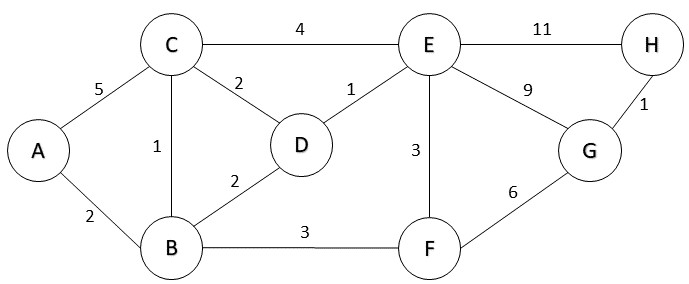
\includegraphics[width=120mm]{undirected_graph2.png}
	\caption{Ένα μη κατευθυνόμενο γράφημα 8 κορυφών με βάρη στις ακμές του}
	\label{fig:undirected_graph2}
\end{figure}

Ο ακόλουθος πίνακας δείχνει την εκτέλεση του αλγορίθμου
\begin{table}[ht!]
	\centering
	\label{tbl:dijkstra3}
	\begin{tabular}{|c|c|c|c|c|c|c|c|c|}
		\hline
		Σύνολο $S$            & A & B        & C        & D        & E        & F        & G        & H         \\ \hline
		$\{\}$                & 0 & $\infty$ & $\infty$ & $\infty$ & $\infty$ & $\infty$ & $\infty$ & $\infty$  \\ \hline
		$\{A\}$               & 0 & $2_A$    & $5_A$    & $\infty$ & $\infty$ & $\infty$ & $\infty$ & $\infty$  \\ \hline
		$\{A,B\}$             & 0 & $2_A$    & $3_B$    & $\infty$ & $\infty$ & $5_B$    & $\infty$ & $\infty$  \\ \hline
		$\{A,B,C\}$           & 0 & $2_A$    & $3_B$    & $4_B$    & $7_C$    & $5_B$    & $\infty$ & $\infty$  \\ \hline
		$\{A,B,C,D\}$         & 0 & $2_A$    & $3_B$    & $4_B$    & $5_D$    & $5_B$    & $\infty$ & $\infty$  \\ \hline
		$\{A,B,C,D,E\}$       & 0 & $2_A$    & $3_B$    & $4_B$    & $5_D$    & $5_B$    & $14_E$   & $16_E$    \\ \hline			
		$\{A,B,C,D,E,F\}$     & 0 & $2_A$    & $3_B$    & $4_B$    & $5_D$    & $5_B$    & $11_F$   & $16_E$    \\ \hline			
		$\{A,B,C,D,E,F,G\}$    & 0 & $2_A$    & $3_B$    & $4_B$    & $5_D$    & $5_B$    & $11_F$   & $12_E$    \\ \hline			
		$\{A,B,C,D,E,F,G,H\}$ & 0 & $2_A$    & $3_B$    & $4_B$    & $5_D$    & $5_B$    & $11_F$   & $12_E$    \\ \hline
	\end{tabular}
	\caption{Συνοπτική εκτέλεση του αλγορίθμου}
\end{table}


Οι συντομότερες διαδρομές είναι:
\begin{itemize}[noitemsep]
\item Για την κορυφή A η διαδρομή είναι η A με μήκος 0
\item Για την κορυφή B η διαδρομή είναι η A-B με μήκος 2
\item Για την κορυφή C η διαδρομή είναι η A-B-C με μήκος 3
\item Για την κορυφή D η διαδρομή είναι η A-B-D με μήκος 4
\item Για την κορυφή E η διαδρομή είναι η A-B-D-E με μήκος 5
\item Για την κορυφή F η διαδρομή είναι η A-B-F με μήκος 5
\item Για την κορυφή G η διαδρομή είναι η A-B-F-G με μήκος 11
\item Για την κορυφή H η διαδρομή είναι η A-B-F-G-H με μήκος 12
\end{itemize}

\subsection{Παράδειγμα 2}
Γράψτε πρόγραμμα που να διαβάζει ένα γράφημα και να εμφανίζει για κάθε κορυφή το βαθμό της, δηλαδή το πλήθος των κορυφών με τις οποίες συνδέεται απευθείας καθώς και το μέσο όρο βαρών για αυτές τις ακμές. Επιπλέον για κάθε κορυφή να εμφανίζει τις υπόλοιπες κορυφές οι οποίες μπορούν να προσεγγιστούν με διαδρομές μήκους 1,2,3 κοκ.

\lstinputlisting[caption = (lab08\_ex2.cpp),multicols=2]{lab08/lab08_ex2.cpp}

Η μεταγλώττιση και η εκτέλεση του κώδικα γίνεται με τις ακόλουθες εντολές:

\lstinputlisting[style=DOS]{lab08/compile_execute3.txt}

Η δε έξοδος που παράγεται είναι η ακόλουθη:

\lstinputlisting[style=DOS]{lab08/lab08_ex2.out}

\section{Ασκήσεις}
\begin{enumerate}[nolistsep]
	\item Υλοποιήστε τον αλγόριθμο των Bellman-Ford \cite{brilliant_bellman_ford} για την εύρεση της συντομότερης διαδρομής από μια κορυφή προς όλες τις άλλες κορυφές.
	\item Υλοποιήστε έναν αλγόριθμο τοπολογικής ταξινόμησης για DAGs \cite{g4g_topological_sort}.
\end{enumerate}

\begin{thebibliography}{9}
\bibitem{g4g_graph_representations}
Geeks for Geeks, graphs and its representations, \href{https://www.geeksforgeeks.org/graph-and-its-representations/}{https://www.geeksforgeeks.org/graph-and-its-representations/}

\bibitem{he_graph_representations}
HackerEarth, graph representation, \href{https://www.hackerearth.com/practice/algorithms/graphs/graph-representation/tutorial/}{https://www.hackerearth.com/practice/algorithms/graphs/graph-representation/tutorial/}

\bibitem{pa_floyd_warshall}
Programming-Algorithms.net, Floyd-Warshall algorithm, \href{http://www.programming-algorithms.net/article/45708/Floyd-Warshall-algorithm}{http://www.programming-algorithms.net/article/45708/Floyd-Warshall-algorithm}

\bibitem{programiz_prim}
PROGRAMIZ, Prim's algorithm, \href{https://www.programiz.com/dsa/prim-algorithm}{https://www.programiz.com/dsa/prim-algorithm}

\bibitem{programiz_kruskal}
PROGRAMIZ, Kruskal's algorithm, \href{https://www.programiz.com/dsa/kruskal-algorithm}{https://www.programiz.com/dsa/kruskal-algorithm}

\bibitem{g4g_topological_sort}
Geeks for Geeks, topological sorting, \href{https://www.geeksforgeeks.org/topological-sorting/}{https://www.geeksforgeeks.org/topological-sorting/}

\bibitem{dicretetext_euler_path}
Discrete Mathematics: An open introduction by Oscar Levin, Euler Paths and Circuits, \href{http://discretetext.oscarlevin.com/dmoi/sec_paths.html}{http://discretetext.oscarlevin.com/dmoi/sec\_paths.html}

\bibitem{he_scc}
HackerEarth, Strongly Connected Components, \href{https://www.hackerearth.com/practice/algorithms/graphs/strongly-connected-components/tutorial/}{https://www.hackerearth.com/practice/algorithms/graphs/strongly-connected-components/tutorial/}

\bibitem{brilliant_bellman_ford}
Brilliant.org, Bellman-Ford Algorithm, \href{https://brilliant.org/wiki/bellman-ford-algorithm/}{https://brilliant.org/wiki/bellman-ford-algorithm/}

\bibitem{algorithm_visualization_dijkstra}
Algorithm visualization, Dijkstra's shortest path, \href{https://www.cs.usfca.edu/~galles/visualization/Dijkstra.html}{https://www.cs.usfca.edu/~galles/visualization/Dijkstra.html}

\end{thebibliography}


% Εργαστήριο 8
\chapter{Δένδρα}
\section{Εισαγωγή}
Τα δένδρα όπως και τα γραφήματα είναι μη γραμμικές δομές δεδομένων που αποτελούν συλλογές κόμβων. Τα δένδρα επιτρέπουν ιεραρχική οργάνωση των δεδομένων όπως φαίνεται στο Σχήμα \ref{fig:binary_tree}. Αυτό το στοιχείο τους επιτρέπει να έχουν καλύτερες επιδόσεις προσπέλασης των επιμέρους στοιχείων σε σχέση με τις γραμμικές λίστες. Με κατάλληλη διευθέτηση των στοιχείων ενός δένδρου καθώς και με εφαρμογή προχωρημένων μηχανισμών εισαγωγής και διαγραφής στοιχείων ο χρόνος εκτέλεσης των περισσότερων λειτουργιών σε ένα δένδρο (ισοζυγισμένο δυαδικό δένδρο αναζήτησης) γίνεται $O(\log n)$. Στην STL τα δένδρα χρησιμοποιούνται στην υλοποίηση των containers std::map και std::set.

\begin{figure}[htbp]
  \centering
  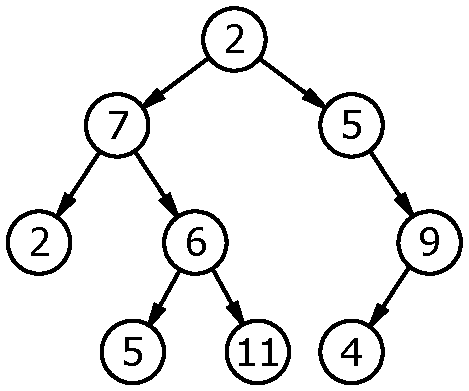
\includegraphics[width=80mm]{Binary_tree.pdf}
  \caption{Ένα απλό δένδρο \cite{wikipedia_binary_tree}}
  \label{fig:binary_tree}
\end{figure}

\section{Δένδρα}

Ένα δένδρο (tree) αποτελείται από κόμβους (nodes) που συνδέονται μεταξύ τους με κατευθυνόμενες ακμές (edges). Ο πρώτος (υψηλότερος) κόμβος του δένδρου ονομάζεται ρίζα (root) ενώ οι κόμβοι που βρίσκονται στα άκρα του δένδρου λέγονται φύλλα (leaves). Οι κόμβοι με τους οποίους συνδέεται απευθείας ένας κόμβος ονομάζονται παιδιά (children) του κόμβου. Αντίστοιχα, ένας κόμβος που έχει παιδιά ονομάζεται γονέας (parent) των αντίστοιχων παιδιών-κόμβων. Απόγονοι (descendants) ενός κόμβου είναι οι κόμβοι για τους οποίους υπάρχει διαδρομή-μονοπάτι (path) πραγματοποιώντας διαδοχικές μεταβάσεις από γονείς σε παιδιά. Αντίστοιχα ορίζεται και η έννοια των προγόνων (ancestors) ενός κόμβου με τη ρίζα να είναι ο μοναδικός κόμβος που δεν έχει προγόνους. 

Τα δένδρα είναι αναδρομικές δομές από τη φύση τους. Κάθε κόμβος ενός δένδρου ορίζει έναν αριθμό από μικρότερα δένδρα, ένα για κάθε παιδί του. Σε ένα δένδρο με $N$ κόμβους υπάρχουν πάντα $N-1$ ακμές καθώς όλοι οι κόμβοι εκτός από τον κόμβο ρίζα έχουν μια ακμή η οποία τους συνδέει με τον γονέα τους.

Το μήκος ενός μονοπατιού ανάμεσα σε δύο κόμβους είναι ίσο με το πλήθος των ακμών του μονοπατιού. Εφόσον υπάρχει μονοπάτι μέσω του οποίου συνδέονται δύο κόμβοι το μονοπάτι αυτό είναι μοναδικό. Για κάθε κόμβο ορίζεται ως \textbf{βάθος του κόμβου} (depth) το μήκος του μονοπατιού από τη ρίζα του δένδρου μέχρι τον ίδιο τον κόμβο. Αντίστοιχα, \textbf{ύψος ενός κόμβου} (height) είναι το μήκος του μακρύτερου μονοπατιού από τον κόμβο προς ένα από τα φύλλα του δένδρου για τα οποία υφίσταται μονοπάτι με αφετηρία τον κόμβο.


\section{Δυαδικά δένδρα}

Δυαδικό δένδρο είναι ένα δένδρο για το οποίο ισχύει ότι κάθε κόμβος έχει το πολύ δύο παιδιά \cite{parlante_binary_tree}. Ένα δένδρο μπορεί να διανυθεί με διαφορετικούς τρόπους. Ορισμένοι βασικοί τρόποι διάσχισης (traversal) του δένδρου παρουσιάζονται στη συνέχεια \cite{g4g_traversals}.

\subsection{Αναζήτηση κατά βάθος}

Η αναζήτηση κατά βάθος (DFS = Depth First Search) διανύει το δένδρο αναζήτησης εξαντλώντας μονοπάτια από τη ρίζα προς τα φύλλα του δένδρου. Ένας τρόπος για να επιτευχθεί αυτό είναι η χρήση αναδρομής. 

\subsubsection{Προ-διατακτική αναζήτηση κατά βάθος}

Στη διάσχιση του δένδρου προ-διατακτικά (pre-order) πρώτα πραγματοποιείται η επίσκεψη στη ρίζα και μετά καλείται αναδρομικά η ίδια συνάρτηση πρώτα για το αριστερό υποδένδρο και μετά για το δεξιό υποδένδρο. 
Συνηθισμένες χρήσεις της pre-order διάσχισης είναι η δημιουργία αντιγράφων ενός δένδρου καθώς και η λήψη της prefix μορφής ενός expression tree \cite{wikipedia_polish_notation}.

\subsubsection{Ένδο-διατακτική αναζήτηση κατά βάθος}

Στη διάσχιση του δένδρου ένδο-διατακτικά (in-order) καλείται αναδρομικά η συνάρτηση για το αριστερό υποδένδρο, μετά πραγματοποιείται επίσκεψη στη ρίζα και μετά καλείται αναδρομικά η συνάρτηση για το δεξιό υποδένδρο.
Εφόσον το δένδρο είναι δυαδικό δένδρο αναζήτησης, η in-order διάσχιση επιστρέφει τους κόμβους σε μη φθίνουσα σειρά. Σχετικά με το τι είναι τα δυαδικά δένδρα αναζήτησης δείτε την παράγραφο~\ref{bst}).

\subsubsection{Μέτα-διατακτική αναζήτηση κατά βάθος}

Στη διάσχιση του δένδρου μέτα-διατακτικά (post-order) πρώτα καλείται αναδρομικά η  συνάρτηση για το αριστερό υποδένδρο, μετά καλείται αναδρομικά για το δεξιό υποδένδρο και τέλος πραγματοποιείται η επίσκεψη στη ρίζα. 
Συνηθισμένες χρήσεις της post-order διάσχισης είναι η διαγραφή ενός δένδρου καθώς και η λήψη της postfix μορφής ενός expression tree \cite{wikipedia_reverse_polish_notation}.

\subsection{Αναζήτηση κατά πλάτος}

Στην αναζήτηση κατά πλάτος (BFS=Breadth First Search) οι κόμβοι του δένδρου διανύονται κατά επίπεδα ξεκινώντας από τη ρίζα και μεταβαίνοντας από πάνω προς τα κάτω. Σε κάθε επίπεδο η προσπέλαση στους κόμβους γίνεται από αριστερά προς τα δεξιά. Για να επιτευχθεί αυτό το είδος διάσχισης του δένδρου χρησιμοποιείται μια ουρά (queue) στην οποία μόλις εξετάζεται ένα στοιχείο προστίθενται στο πίσω άκρο της ουράς τα παιδιά του.

\lstinputlisting[caption = header file για το δυαδικό δένδρο (binary\_tree.hpp)]{lab09/binary_tree.hpp}

\lstinputlisting[caption = source file για το δυαδικό δένδρο αναζήτησης (binary\_tree.cpp),multicols=2]{lab09/binary_tree.cpp}

Ο ακόλουθος κώδικας δημιουργεί το δυαδικό δένδρο του Σχήματος~\ref{fig:binary_tree1}.

\begin{figure}[htbp]
  \centering
  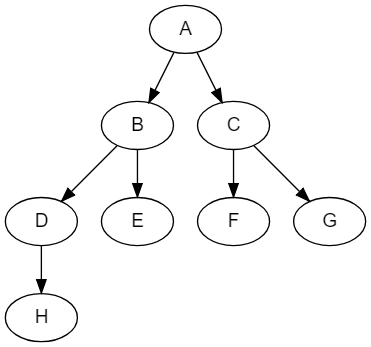
\includegraphics[width=80mm]{binary_tree1.png}
  \caption{Δυαδικό δένδρο με λεκτικά ως τιμές κλειδιών στους κόμβους}
  \label{fig:binary_tree1}
\end{figure}

\lstinputlisting[caption = Δοκιμή των συναρτήσεων του δυαδικού δένδρου (binary\_tree\_ex1.cpp)]{lab09/binary_tree_ex1.cpp}

Η μεταγλώττιση και η εκτέλεση του κώδικα γίνεται με τις ακόλουθες εντολές:

\lstinputlisting[style=DOS]{lab09/compile_execute1.txt}

Η δε έξοδος που παράγεται και για τους 4 τρόπους διάσχισης του δένδρου είναι η ακόλουθη:

\lstinputlisting[style=DOS]{lab09/binary_tree_ex1.out}


\section{Δυαδικά δένδρα αναζήτησης}
\label{bst}
Σε ένα δυαδικό δένδρο αναζήτησης θα πρέπει να ισχύει ότι για κάθε κόμβο όλες οι τιμές κλειδιών στο δένδρο αριστερά του κόμβου θα πρέπει να είναι μικρότερες από την τιμή κλειδιού του κόμβου. Αντίστοιχα, όλες οι τιμές κλειδιών στο δένδρο δεξιά του κάθε κόμβου θα πρέπει να είναι μεγαλύτερες από την τιμή κλειδιού του κόμβου.

\subsection{Υλοποίηση δυαδικού δένδρου αναζήτησης}

Ιδιαίτερη προσοχή θα πρέπει να δοθεί στην υλοποίηση της διαγραφής ενός κόμβου από το δένδρο έτσι ώστε το δένδρο και μετά τη διαγραφή να εξακολουθεί να είναι δυαδικό δένδρο αναζήτησης \cite{jumping_into_cpp}. 

\begin{figure}[!tbp]
  \centering
  \begin{minipage}[b]{0.4\textwidth}
    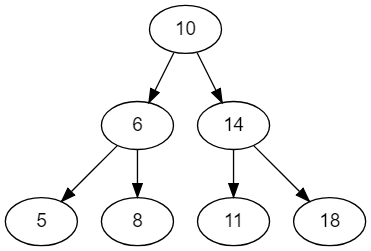
\includegraphics[width=\textwidth]{bst1.png}
    \label{fig:bst1}
    \caption{Δυαδικό δένδρο αναζήτησης}
  \end{minipage}
  \hfill
  \begin{minipage}[b]{0.4\textwidth}
    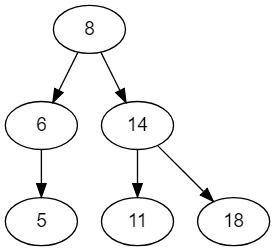
\includegraphics[width=\textwidth]{bst2.png}
    \label{fig:bst2}
    \caption{Το δυαδικό δένδρο αναζήτησης μετά τη διαγραφή της ρίζας}
  \end{minipage}
\end{figure}

\lstinputlisting[caption = header file για το δυαδικό δένδρο αναζήτησης (bst.hpp)]{lab09/bst.hpp}

\lstinputlisting[caption = source file για το δυαδικό δένδρο αναζήτησης (bst.cpp),multicols=2]{lab09/bst.cpp}

\lstinputlisting[caption = Δοκιμή των συναρτήσεων του δυαδικού δένδρου αναζήτησης (bst\_ex1.cpp),multicols=2]{lab09/bst_ex1.cpp}

Η μεταγλώττιση και η εκτέλεση του κώδικα γίνεται με τις ακόλουθες εντολές:

\lstinputlisting[style=DOS]{lab09/compile_execute2.txt}

Η δε έξοδος που παράγεται είναι η ακόλουθη:

\lstinputlisting[style=DOS]{lab09/bst_ex1.out}

Για να πραγματοποιηθεί η διαγραφή του κόμβου 10, εντοπίζεται ο κόμβος με τη μεγαλύτερη τιμή στο αριστερό υποδένδρο του κόμβου 10, που είναι ο 8 και ο κόμβος αυτός αφαιρείται από το δένδρο αντικαθιστώντας τον κόμβο 10.

\section{Ισοζυγισμένα δυαδικά δένδρα αναζήτησης}
\label{bbst}

Οι καλές επιδόσεις ενός δυαδικού δένδρου αναζήτησης χάνονται όταν το δένδρο δεν είναι ισοζυγισμένο (balanced), δηλαδή όταν υπάρχουν μονοπάτια από τη ρίζα προς τα φύλλα με μεγάλα βάθη ενώ άλλα μονοπάτια έχουν μικρά βάθη. Υπάρχουν διάφορες μορφές ισοζυγισμένων δένδρων με πλέον δημοφιλή τα κόκκινα-μαύρα δένδρα (red black trees) και τα AVL (Adelson, Velskii και Landis) δένδρα. Σε αυτά τα δένδρα πραγματοποιούνται ειδικές λειτουργίες (περιστροφές) έτσι ώστε κατά την εισαγωγή νέων τιμών στο δένδρο και τη διαγραφή τιμών από το δένδρο, τα βάθη των φύλλων του δένδρου εγγυημένα να διατηρούνται σε κοντινές τιμές μεταξύ τους. Ισχύει ότι τα AVL δένδρα είναι καλύτερα ισοζυγισμένα από τα κόκκινα-μαύρα δένδρα αλλά έχουν το μειονέκτημα της υψηλότερης υπολογιστικής επιβάρυνσης κατά την εισαγωγή και τη διαγραφή κόμβων.

\section{Παραδείγματα}

\subsection{Παράδειγμα 1}

Δεδομένου ενός δυαδικού δένδρου ζητείται η εκτύπωση όλων των διαδρομών από τη ρίζα του δένδρου μέχρι κάθε φύλλο. Για παράδειγμα, για το δένδρο του Σχήματος~\ref{fig:binary_tree1} το πρόγραμμα θα πρέπει να επιστρέψει ABDH, ABE, ACF και ACG.

\lstinputlisting[caption = Λύση παραδείγματος 1 (lab09\_ex1.cpp),multicols=2]{lab09/lab09_ex1.cpp}

Η μεταγλώττιση και η εκτέλεση του κώδικα γίνεται με τις ακόλουθες εντολές:

\lstinputlisting[style=DOS]{lab09/compile_execute3.txt}

Η έξοδος που παράγεται είναι η ακόλουθη:

\lstinputlisting[style=DOS]{lab09/lab09_ex1.out}


\subsection{Παράδειγμα 2}

Δεδομένου ενός δυαδικού δένδρου ζητείται να πραγματοποιείται έλεγχος σχετικά με το εάν το δένδρο είναι δυαδικό δένδρο αναζήτησης ή όχι. 

\lstinputlisting[caption = Λύση παραδείγματος 2 (lab09\_ex2.cpp),multicols=2]{lab09/lab09_ex2.cpp}

Η μεταγλώττιση και η εκτέλεση του κώδικα γίνεται με τις ακόλουθες εντολές:

\lstinputlisting[style=DOS]{lab09/compile_execute4.txt}

Η έξοδος που παράγεται είναι η ακόλουθη:

\lstinputlisting[style=DOS]{lab09/lab09_ex2.out}

\section{Ασκήσεις}

\begin{enumerate}[nolistsep]
\item Να γράψετε πρόγραμμα που να εμφανίζει τους κόμβους ενός δυαδικού δένδρου κατά επίπεδα από κάτω προς τα πάνω και από αριστερά προς τα δεξιά. Δηλαδή στο δένδρο του Σχήματος \ref{fig:binary_tree1} θα πρέπει οι κόμβοι να εμφανιστούν ως D, E, F, G, B, C, A.
\item Να γράψετε πρόγραμμα που να δημιουργεί από έναν ταξινομημένο πίνακα ακεραίων ένα δυαδικό δένδρο αναζήτησης. Να χρησιμοποιηθεί ο ακόλουθος αλγόριθμος:
	\begin{enumerate}[nolistsep]
	\item Εύρεση του μεσαίου στοιχείου του πίνακα και ορισμός του ως ρίζα του δένδρου
	\item Αναδρομική εκτέλεση για το αριστερό και το δεξιό μισό
		\begin{enumerate}[nolistsep]
		\item Εύρεση του μεσαίου στοιχείου του αριστερού μέρους και ορισμός του ως 		αριστερό παιδί της ρίζας του βήματος α'
		\item Εύρεση του μεσαίου στοιχείου του δεξιού μέρους και ορισμός του ως δεξί παιδί της ρίζας του βήματος α'
		\end{enumerate}
	\end{enumerate}
\end{enumerate}

\begin{thebibliography}{9}
\bibitem{wikipedia_binary_tree}
Wikipedia, Tree (data structure), \href{https://en.wikipedia.org/wiki/Tree_(data_structure)}{https://en.wikipedia.org/wiki/Tree\_(data\_structure)}

\bibitem{parlante_binary_tree}
Binary Trees by Nick Parlante, \href{http://cslibrary.stanford.edu/110/BinaryTrees.html}{http://cslibrary.stanford.edu/110/BinaryTrees.html}

\bibitem{wikipedia_polish_notation}
Wikipedia, Polish Notation, \href{https://en.wikipedia.org/wiki/Polish_notation}{https://en.wikipedia.org/wiki/Polish\_notation}

\bibitem{wikipedia_reverse_polish_notation}
Wikipedia, Reverse Polish Notation, \href{https://en.wikipedia.org/wiki/Reverse_Polish_notation}{https://en.wikipedia.org/wiki/Reverse\_Polish\_notation}

\bibitem{g4g_traversals}
Tree Traversals (Inorder, Preorder and Postorder), \href{https://www.geeksforgeeks.org/tree-traversals-inorder-preorder-and-postorder/}{https://www.geeksforgeeks.org/tree-traversals-inorder-preorder-and-postorder/}

\bibitem{jumping_into_cpp}
Alex Allain, Jumping into C++, cprogramming.com, Chapter 17 - Binary Trees, 2013

\end{thebibliography}




\end{document}

